\documentclass[conference]{IEEEtran}

\usepackage[usenames,dvipsnames,svgnames,table]{xcolor}
\usepackage{amsmath}
\usepackage{amsfonts}
\usepackage{cite}
\usepackage{graphicx}
\usepackage{listings}
\usepackage{multirow}
\usepackage{tabularx}
\usepackage{varioref}
\usepackage{hyperref}
\usepackage[noabbrev,capitalize]{cleveref}
\usepackage[group-separator={,}, group-four-digits=true]{siunitx}
\usepackage{lscape}
\usepackage{bm}
\usepackage{chngpage}
\usepackage{blindtext} % For filler text

\usepackage[english]{babel}
\usepackage[utf8]{inputenc}

%Includes "References" in the table of contents
\usepackage[nottoc]{tocbibind}


\lstset{
  frame=single,
  basicstyle=\ttfamily,% print whole listing small
  language=R,
  aboveskip=3mm,
  belowskip=3mm,
  showstringspaces=false,
  columns=flexible,
  numbers=none,
  commentstyle=\color{ForestGreen},
  stringstyle=\color{Maroon},
  breaklines=true,
  breakatwhitespace=true,
  tabsize=2,
  literate={<-}{{$\gets$}}1 {~}{{$\sim$}}1
}

\hypersetup{
  colorlinks=true,
  linkcolor=blue,
  urlcolor=blue,
}

\sisetup{output-exponent-marker=\textsc{e}}

\begin{document}

\title{Machine Learning Project Proposal}
\author{\IEEEauthorblockN{William Clark}
\IEEEauthorblockA{will.clark@chicagobooth.edu\\
University of Chicago Booth School of Business}
\and
\IEEEauthorblockN{Matthew DeLio}
\IEEEauthorblockA{mdelio@chicagobooth.edu\\
University of Chicago Booth School of Business}}

\maketitle

\section{Summary}
For our final project we will enter a Kaggle contest called \textbf{Facial Keypoints Detection}. The goal of the contest is to predict the $(x,y)$ coordinates of the following facial keypoints for a given set of portrait pictures:
\begin{itemize}
\item center of each eye (2),
\item inner and outer corner of each eye (4),
\item end of each eyebrow (4),
\item tip of nose (1),
\item corners of mouth (2), and
\item center of each lip (2),
\end{itemize}
for a total of 15 features per face. Our submission will be scored by the average root mean square error (RMSE) across all keypoints and images.

\section{Data Set}
Our data are a set of \num{8832} 96-by-96 grayscale images of tightly cropped portraits (sample images are shown in \cref{fig:sample_faces}). The images have been vectorized and each pixel is represented by its grayscale intensity on a $(0,255)$ scale. The $(x,y)$ coordinates of all facial keypoints are given, so there are 30 variables to predict for each image. Our models/algorithms will be tested on a testing set of \num{1783} similarly formatted images.
\begin{figure}[!ht]
\centering
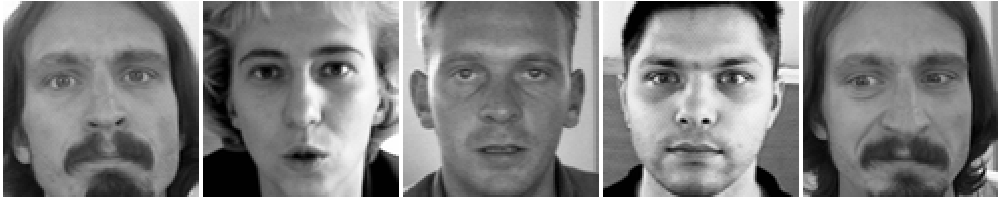
\includegraphics[width=3.5in]{sample_faces.pdf}
\caption{Sample Faces in Training Data Set}
\label{fig:sample_faces}
\end{figure}

\section{Project Description}
This project can be thought of in two discrete parts: (1) image preprocessing to reduce the dimensionality of our data set and make our modeling efforts more robust, and (2) a predictive modeling exercise to identify facial keypoints.

\subsection{Image Processing}
A common practice in other computer vision studies is to use principal components analysis to reduce the dimensionality of the images. In most cases, nearly all the variation across images can be explained with a fraction of the original data set. Rather than defining each image as a vector of length $p=96\cdot96$, we can express it as a linear combination of the first $x$ principal components where $x \ll p$. This process should reduce the noise in each vectorized image and increase the accuracy of the predictive algorithms we need to train and tune.

\textbf{TODO (mdelio): drop some domain specific knowledge}

\subsection{Predictive Modeling}
This project requires training and tuning 30 different predictive algorithms/models, one for each $x$ and $y$ coordinate of all 15 facial features. The following list of models/algorithms is neither exclusive nor exhaustive, but represents our best current estimate of what the final paper might include:
\begin{itemize}
\item linear regression with L1/L2 penalization,
\item nearest neighbor searches,
\item regression trees and bagged regression trees,
\item random forests,
\item boosting trees, and
\item neural networks.
\end{itemize}
With this variety of forecasting models, we could make our prediction based on the best performing model or best performing set of models (such that our final algorithm is an ensemble of some combination of listed models).

\end{document}


